\documentclass[conference]{IEEEtran}
\IEEEoverridecommandlockouts
 
\usepackage[utf8]{inputenc}
\usepackage[spanish]{babel}
\usepackage{cite}
\usepackage{amsmath,amssymb,amsfonts}
\usepackage{graphicx}
\usepackage{textcomp}
\usepackage{xcolor}
\usepackage{hyperref}
\usepackage{booktabs}
\usepackage{float}
\usepackage{tikz}
\usetikzlibrary{shapes.geometric,arrows.meta,positioning,fit,backgrounds}
 
\definecolor{mlopsblue}{RGB}{31,78,121}
\definecolor{mlopsgreen}{RGB}{0,97,0}
\definecolor{mlopsorange}{RGB}{180,95,6}
\definecolor{mlopsgray}{RGB}{80,80,80}
\definecolor{mlopslight}{RGB}{220,230,242}
\definecolor{mlopspurple}{RGB}{106,61,154}
\definecolor{mlopspurplelight}{RGB}{232,224,242}
\definecolor{mlopsteal}{RGB}{0,105,92}
\definecolor{mlopstealight}{RGB}{204,232,229}
 
\def\BibTeX{{\rm B\kern-.05em{\sc i\kern-.025em b}\kern-.08em
    T\kern-.1667em\lower.7ex\hbox{E}\kern-.125emX}}
 
\begin{document}

%=============================================================
%  TÍTULO Y AUTORES
%=============================================================
\title{Sistema Predictivo con MLOps para la Estimación de Carga de\\
Trabajo y Producción en Cosechas Humano--Robot}

\author{
\IEEEauthorblockN{Ivan García Fernández}
\IEEEauthorblockA{\textit{Facultad de ingeniería}\\
\textit{ Universidad Andres Bello}\\
 Santiago, Chile.\\
i.garciafernandez@uandresbello.edu}
}

\maketitle

%=============================================================
%  ABSTRACT
%=============================================================
\begin{abstract}
La creciente incorporación de robots colaborativos en entornos agrícolas genera desafíos inéditos para la planificación operativa de las cosechas. Este trabajo propone el diseño e implementación de un sistema predictivo basado en \textit{machine learning} (ML) que estima la carga de trabajo humano (\textit{workload}) y la producción total recolectada en dos escenarios contrastados: cosecha exclusivamente manual y cosecha con apoyo robótico. Los datos provienen de simulaciones MATLAB con diseño experimental factorial, en las que se modelan agentes con máquinas de estado y lógica difusa de navegación. A partir de estas simulaciones, se construye un pipeline que abarca limpieza de datos, análisis estadístico multifactorial (ANOVA), selección de variables y comparación de modelos de regresión supervisada. El modelo óptimo se integra en una arquitectura MLOps que contempla el versionado de experimentos con MLflow sobre backend PostgreSQL, la exposición del modelo como servicio REST con FastAPI genérico multi-experimento, autenticación y TLS (Keycloak/OAuth2 y \textit{API keys}), observabilidad con Prometheus y Grafana, y contenedorización con Docker, garantizando reproducibilidad en un entorno de testing similar a producción validado mediante una pirámide de pruebas de seis niveles. El sistema constituye una contribución en el cruce entre sistemas inteligentes aplicados a agricultura de precisión y prácticas modernas de ingeniería de software para el despliegue de modelos ML.
\end{abstract}
 
\begin{IEEEkeywords}
MLOps, machine learning, cosecha agrícola, interacción humano--robot, predicción de workload, FastAPI, MLflow, Docker, simulación MATLAB
\end{IEEEkeywords}
 
%=============================================================
%  I. INTRODUCCIÓN
%=============================================================
\section{Introducción}
 
\subsection{Contexto: agricultura, robótica e IA}
 
La agricultura enfrenta presiones estructurales que impulsan la adopción acelerada de tecnologías de automatización. El envejecimiento de la mano de obra rural, la escasez estacional de trabajadores y la necesidad de maximizar la eficiencia operativa han convertido a los robots agrícolas en una solución con creciente viabilidad técnica y económica \cite{willekens2025}. Revisiones sistemáticas recientes documentan una explosión en el uso de inteligencia artificial (IA) y robótica en agricultura a lo largo de la última década \cite{hamrani2025,aijaz2025}, abarcando tareas que van desde la detección de cultivos y la navegación autónoma \cite{wakchaure2023} hasta la colaboración directa con operadores humanos \cite{adamides2023}.
 
En particular, los sistemas de cosecha semi-autónoma donde personas y robots comparten el espacio de trabajo representan un paradigma emergente con alto potencial productivo \cite{benos2023hri}. La interacción humano--robot (HRI) en contextos agrícolas introduce variables dinámicas que afectan directamente la productividad y la seguridad: el número de trabajadores, el ritmo de cosecha, la distribución espacial de la plantación, el tipo de actividad asignada y el nivel de utilización del robot \cite{guevara2024}. La referencia base de este proyecto, Vásconez y Auat Cheein \cite{vasconez2022}, desarrolló simulaciones multiagente de cosecha en huertos y demostró que la colaboración humano--robot mejora la eficiencia operativa de manera significativa; sin embargo, no propone modelos predictivos que permitan anticipar el comportamiento del sistema bajo distintas configuraciones antes de ejecutarlas en terreno.
 
Revisiones adicionales sobre tendencias en ML y robótica agrícola, sistemas de precisión y colaboración humano--robot confirman el creciente interés por integrar IA en todas las etapas del proceso productivo \cite{halder2026,taha2025,li2024,thakur2025,mohyuddin2024,moysiadis2024,benos2025xai,icoici2024,logeshwaran2024,tgrs2023}.
 
\subsection{ML en agricultura y el problema de datos acotados}
 
El aprendizaje automático ha demostrado ser una herramienta poderosa para la predicción de variables agrícolas a partir de datos operacionales \cite{sharma2023,kuan2025}. Estudios recientes muestran que métodos de \textit{ensemble} como Random Forest y XGBoost ofrecen alto desempeño en tareas de regresión sobre datos tabulares en dominio agrícola \cite{arunkumar2025,sharma2023}. No obstante, un desafío frecuente en este tipo de proyectos es el tamaño acotado del conjunto de datos, ya que los experimentos provienen de simulaciones controladas con variaciones factoriales finitas. Trabajos en dominios relacionados han demostrado que estrategias como la validación k-fold y la regularización permiten obtener modelos robustos en escenarios de datos reducidos \cite{ejss2025}, lo que sustenta la viabilidad del enfoque propuesto.
 
\subsection{La brecha MLOps en agricultura de precisión}
 
A pesar del avance en modelos predictivos, existe una brecha significativa entre el desarrollo experimental de modelos ML y su despliegue como herramientas operativas accesibles y reproducibles. Esta brecha ha dado origen al campo de MLOps (\textit{Machine Learning Operations}), que integra prácticas de ingeniería de software —integración continua, versionado de artefactos, contenedorización— con el ciclo de vida completo de los modelos ML \cite{autodrift2025}. Trabajos recientes demuestran que pipelines MLOps basados en MLflow y Docker permiten construir sistemas de predicción reproducibles, escalables y desplegables en entornos de producción \cite{arunkumar2025,singh2025}. En agricultura de precisión, sin embargo, la adopción de MLOps es aún incipiente: Ozimek et al.\ \cite{ozimek2026} presentan uno de los pocos casos documentados de arquitectura ML desplegada con prácticas CI/CD en agricultura, lo que indica que este cruce representa tanto una necesidad urgente como una oportunidad de contribución concreta.
 
\subsection{Propuesta}
 
El presente proyecto aborda este vacío mediante el desarrollo de un sistema predictivo \textit{end-to-end} que extiende el trabajo de Vásconez y Auat Cheein \cite{vasconez2022} incorporando un pipeline ML completo y una arquitectura MLOps para el despliegue del modelo óptimo. La fuente de datos son simulaciones MATLAB de dos escenarios contrastados —cosecha solo humanos y cosecha humano--robot— bajo un diseño factorial que varía el número de trabajadores, la fila de cultivo, el modo de actividad y la posición inicial. El objetivo es proporcionar una herramienta accesible vía API capaz de anticipar el comportamiento del sistema bajo distintas configuraciones, apoyando decisiones de planificación más informadas, eficientes y reproducibles.
 
%=============================================================
%  II. OBJETIVOS Y PREGUNTAS DE INVESTIGACIÓN
%=============================================================
\section{Objetivos y Preguntas de Investigación}
 
\subsection{Objetivo General}
 
Desarrollar e implementar un sistema predictivo basado en machine learning, desplegado bajo una arquitectura MLOps, capaz de estimar la carga de trabajo humano y la producción cosechada en escenarios de colaboración humano--robot, accesible como servicio REST en un entorno de testing similar a producción.
 
\subsection{Objetivos Específicos}
 
\begin{enumerate}
    \item Preparar y analizar estadísticamente los datos experimentales de simulación (ANOVA multifactorial tipo III), identificando las variables predictoras más relevantes para las cuatro variables objetivo —\textit{Total recolectado}, producción en zona de carga, \textit{Total workload} y producción promedio humana— en ambos escenarios (8 \textit{targets} en total).
    \item Entrenar y comparar múltiples modelos de regresión supervisada evaluando su desempeño mediante métricas estándar (R\textsuperscript{2}, MAE, RMSE) sobre tres conjuntos de variables de entrada distintos.
    \item Implementar una arquitectura MLOps que integre versionado de experimentos (MLflow sobre PostgreSQL) y de datos (DVC), despliegue como API REST genérica (FastAPI), autenticación y TLS (Keycloak/OAuth2, \textit{API key}), observabilidad (Prometheus + Grafana) y contenedorización (Docker), incorporando monitoreo de \textit{drift} con reentrenamiento automático (\textit{champion/challenger}) y pipelines de CI/CD que reemplacen la evaluación manual por un proceso automatizado y reproducible.
    \item Validar el sistema en un entorno de testing basado en \texttt{docker-compose}, mediante una pirámide de pruebas de seis niveles (datos, modelo, API, \textit{performance drift}, \textit{model slices} y contrato de API) que verifique disponibilidad del servicio, reproducibilidad de predicciones, ausencia de sesgo por sub-grupo y correctitud de los resultados.
\end{enumerate}
 
\subsection{Preguntas de Investigación}
 
\begin{itemize}
    \item \textbf{PI-1:} ¿Cuáles variables operativas son más determinantes para predecir workload y producción total según el análisis ANOVA, y difieren entre escenario solo humanos y humano--robot?
    \item \textbf{PI-2:} ¿Qué familia de algoritmos de regresión ofrece el mejor desempeño predictivo dado el tamaño acotado del conjunto de datos generado por las simulaciones?
    \item \textbf{PI-3:} ¿Qué métricas de calidad de servicio (latencia, reproducibilidad entre ejecuciones) alcanza el sistema desplegado en el entorno de testing con contenedores?
\end{itemize}
 
%=============================================================
%  III. METODOLOGÍA
%=============================================================
\section{Metodología}
 
La metodología se organiza en tres bloques secuenciales, tal como se ilustra en la Figura~\ref{fig:arquitectura}. Los Bloques 1 y 2 constituyen el pipeline de análisis estadístico y ML; el Bloque 3 (MLOps) reemplaza la etapa de tabla comparativa final y herramienta predictiva estática del diseño original, sustituyéndola por un pipeline automatizado de registro, despliegue y servicio.
 
Un aspecto clave para la factibilidad es que tanto los datos de simulación como la infraestructura MLOps \textbf{ya se encuentran operativos y en una etapa madura}: los dos escenarios fueron consolidados en \texttt{simulation\_all.csv} (284 observaciones, 8 variables objetivo, versionado con DVC) y, sobre este conjunto, ya están entrenados, registrados y desplegados los 8 modelos de regresión descritos en la Sección~\ref{sec:mlops}, junto con su servicio FastAPI genérico multi-experimento, backend PostgreSQL para MLflow, autenticación TLS/Keycloak/\textit{API key}, observabilidad con Prometheus y Grafana, monitoreo de \textit{drift} y pipelines de CI/CD operando sobre un \textit{runner self-hosted}. La validación de este stack ya se ejecutó al menos una vez de punta a punta mediante la pirámide de pruebas de seis niveles (Sección~\ref{sec:mlops}), lo que arrojó hallazgos concretos aún pendientes de corrección (Sección~\ref{sec:mlops}). Las cinco semanas disponibles se concentran, por lo tanto, en: (i) completar el análisis ANOVA y la comparación de los conjuntos de variables Set~B y Set~C (Sección~\ref{sec:bloque2}), (ii) generar la tabla comparativa final de modelos por escenario y \textit{feature set}, y (iii) corregir los hallazgos de la validación \textit{end-to-end} y volver a certificar el stack bajo el dominio HRI. Esto hace el proyecto no solo factible, sino que reduce el riesgo de ejecución a tareas de análisis y corrección dirigida sobre un sistema ya en operación.
 
%% ---- FIGURA 1: Arquitectura general ----
\begin{figure*}[t]
    \centering
    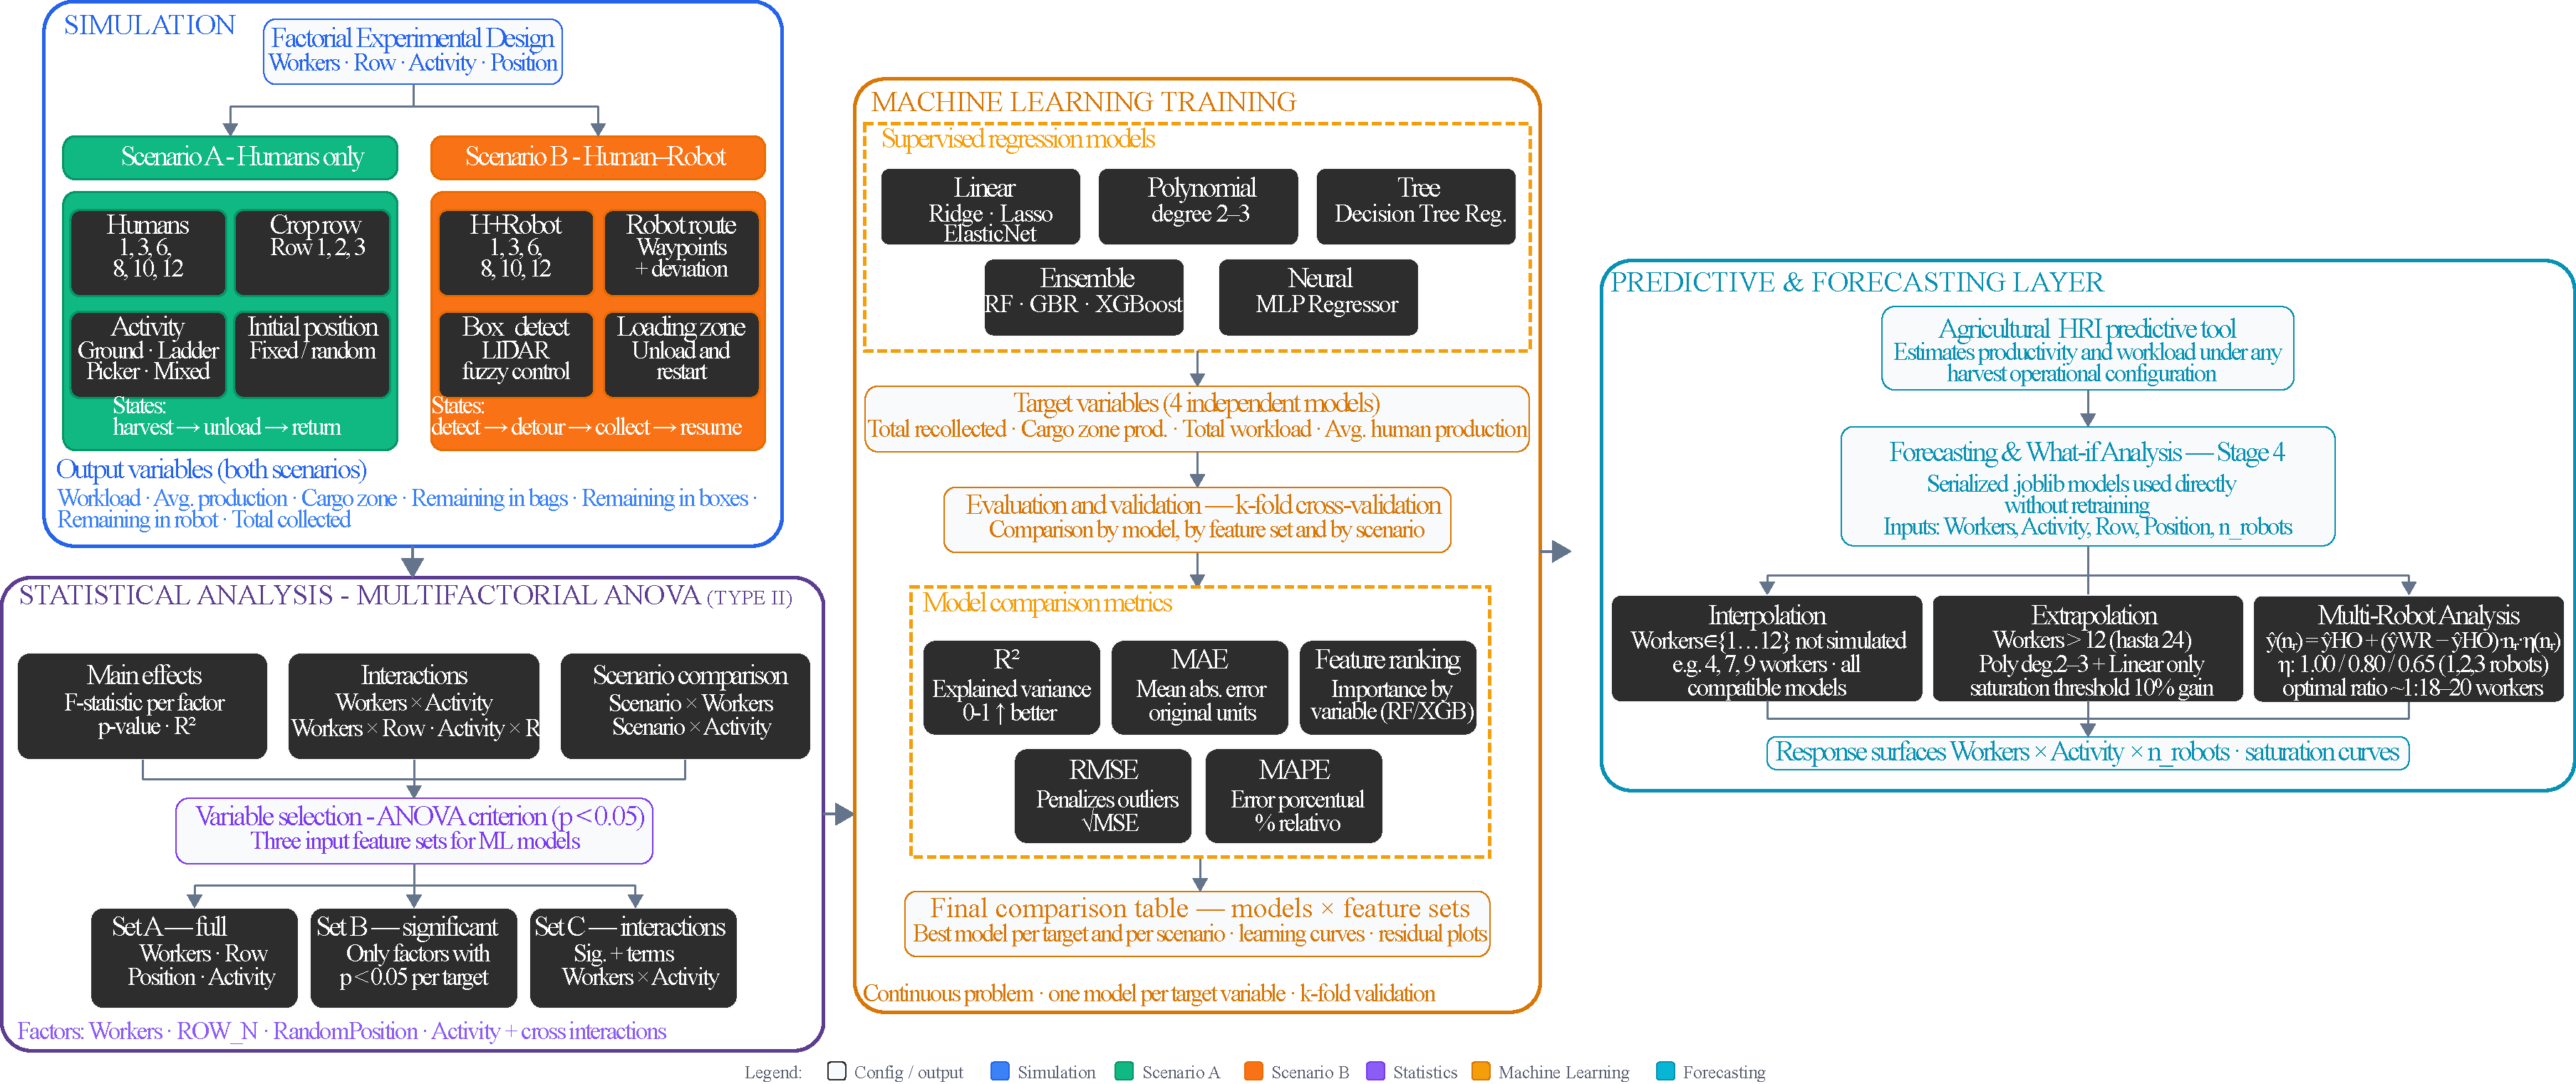
\includegraphics[width=\textwidth]{Arquitectura.pdf}
    \caption{Arquitectura general del sistema. El pipeline cubre desde el diseño experimental factorial y la simulación MATLAB hasta el entrenamiento comparativo de modelos. El bloque MLOps (Sección~\ref{sec:mlops}) reemplaza la etapa de tabla comparativa final, automatizando el registro, despliegue, monitoreo de \textit{drift} y reentrenamiento de los 8 modelos óptimos.}
    \label{fig:arquitectura}
\end{figure*}
 
\subsection{Bloque 1: Descripción de Datos y Preparación}
 
Los datos disponibles provienen de simulaciones MATLAB previamente ejecutadas, con un diseño experimental factorial completo que varía cuatro factores: número de trabajadores (1, 3, 6, 8, 10, 12), fila de cultivo (1--3), modo de actividad (\textit{Ground, Ladder, Picker, Mixed}) y posición inicial (fija/aleatoria). El Escenario A (solo humanos) cuenta con 144 registros y el Escenario B (humano--robot) con 140 registros, consolidados en un único archivo \texttt{simulation\_all.csv} de 284 observaciones y 15 columnas. Los dos escenarios contrastados se describen a continuación.
 
\subsubsection{Escenario A — Cosecha Solo Humanos}
 
Cada trabajador sigue una máquina de estados de seis fases: cosecha en árbol, descenso de escalera, traslado a zona de carga, descarga, retorno al árbol y subida de escalera (Figura~\ref{fig:escenario1}). El costo metabólico se acumula a $dt = 0{,}25$ s, $T = 600$ s según constantes energéticas por actividad ($c_\text{harv}$, $c_\text{ld}$, $c_\text{wlk}$, etc.).
 
%% ---- FIGURA 2: Escenario 1 ----
\begin{figure}[H]
    \centering
    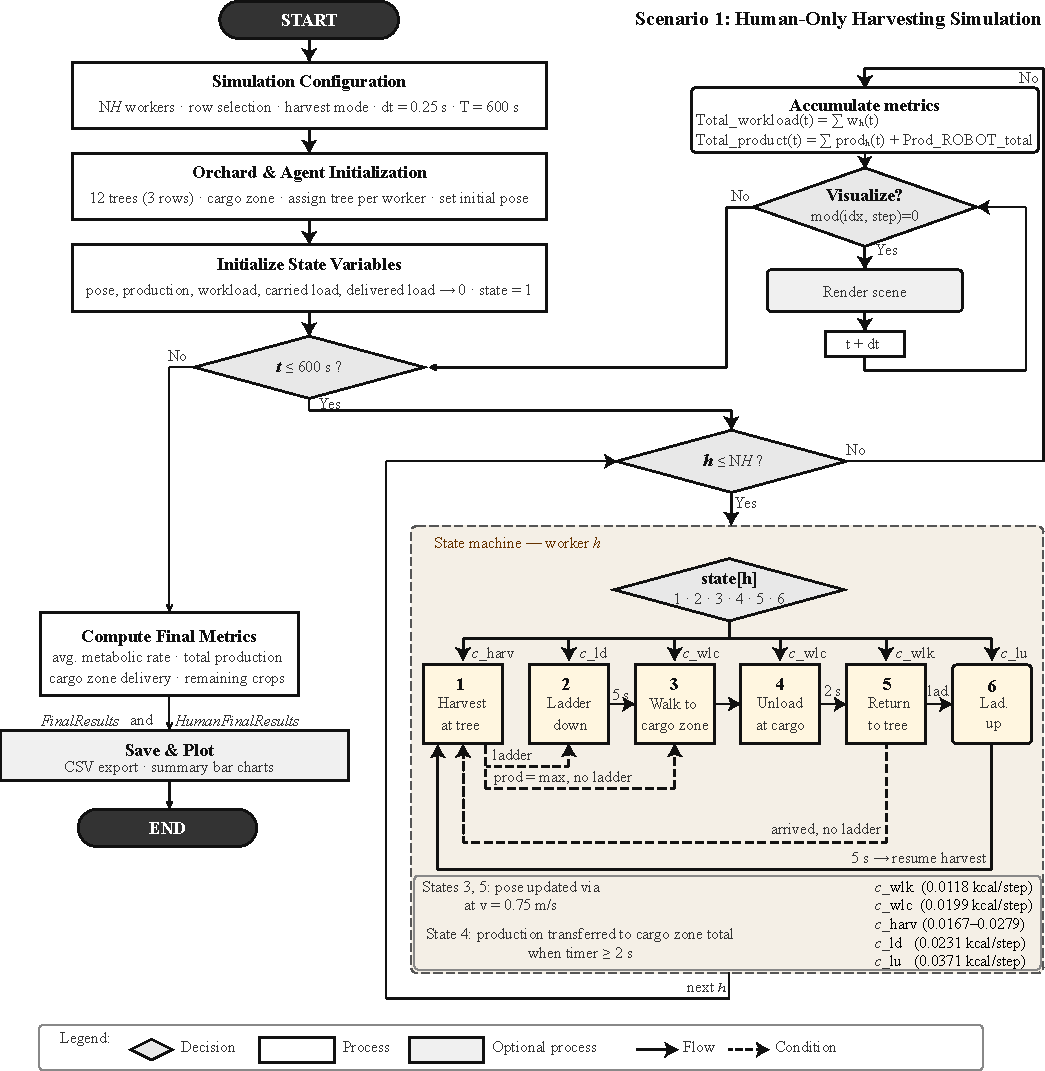
\includegraphics[width=\columnwidth]{flowchart_scenario1_human_harvesting.pdf}
    \caption{Escenario A: simulación de cosecha con agentes humanos únicamente. El trabajador $h$ sigue una máquina de 6 estados que modela el ciclo completo cosecha--traslado--descarga, acumulando carga de trabajo metabólico en cada paso de tiempo.}
    \label{fig:escenario1}
\end{figure}
 
\subsubsection{Escenario B — Cosecha Humano--Robot}
 
Extiende el Escenario A incorporando un robot autónomo con LIDAR (13 haces, $r = 1{,}5$ m) y detector de objetos (FoV~$= 120°$, $r = 3$ m). El robot navega con tres controladores difusos (\texttt{fis\_goal}, \texttt{fis\_obstacle}, \texttt{fis\_tracking}) y rutas PRM, desviándose para recoger cajas de los trabajadores y transportarlas a la zona de carga (Figura~\ref{fig:escenario2}).
 
%% ---- FIGURA 3: Escenario 2 ----
\begin{figure}[H]
    \centering
    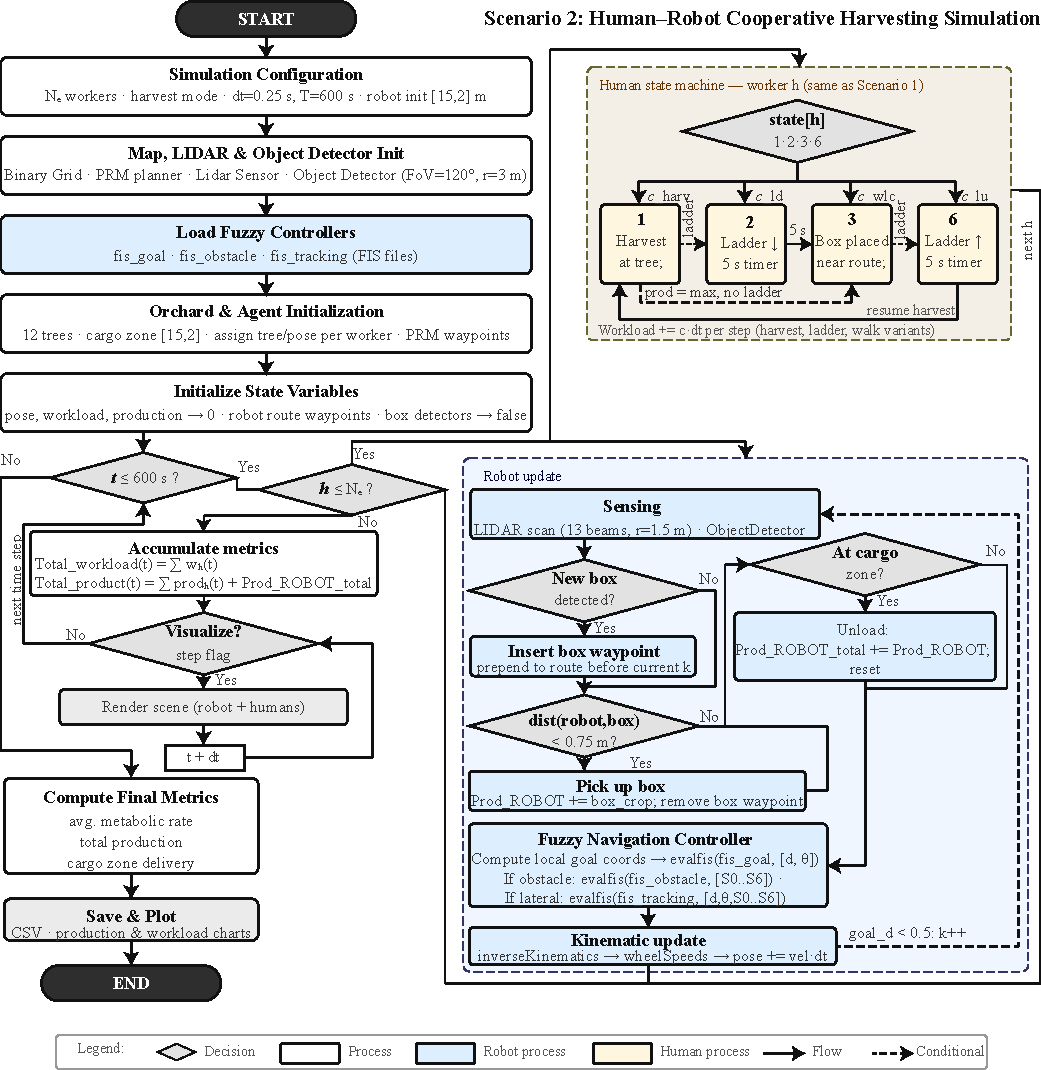
\includegraphics[width=\columnwidth]{flowchart_scenario2_robot_human_harvesting.pdf}
    \caption{Escenario B: simulación de cosecha humano--robot. El robot actualiza su estado mediante LIDAR, detección de cajas, navegación difusa y cinemática inversa, acumulando producción robótica que se suma a la producción humana total.}
    \label{fig:escenario2}
\end{figure}
 
Las cuatro variables objetivo del modelado predictivo —\textit{Total recolectado}, producción en zona de carga, \textit{Total workload} y producción promedio humana— se modelan de forma independiente para cada escenario, totalizando 8 \textit{targets} (Figura~\ref{fig:arquitectura}). Estas variables fueron seleccionadas por su relevancia directa para la planificación operativa: las dos primeras caracterizan el rendimiento productivo de la faena, mientras que \textit{Total workload} y la producción promedio reflejan el esfuerzo y desempeño individual del equipo humano. Las variables predictoras son \texttt{Humans}, \texttt{ROW\_N}, \texttt{RandomPosition} y la actividad codificada \textit{one-hot} (\texttt{Act\_Ladder}, \texttt{Act\_Mixed}, \texttt{Act\_Picker}, con \textit{ground} como categoría base). La preparación de los datos incluye eliminación de registros incompletos, tratamiento de atípicos y normalización de predictores continuos.
 
\subsection{Bloque 2: Análisis Estadístico y Entrenamiento de Modelos}
\label{sec:bloque2}
 
\subsubsection{ANOVA Multifactorial y Selección de Variables}
 
Se aplica ANOVA tipo III sobre factores principales (Workers, ROW\_N, RandomPosition, Activity) e interacciones cruzadas (Workers$\times$Activity, Workers$\times$Row, Activity$\times$Row). Criterio de selección: $p < 0{,}05$. Se construyen tres conjuntos de entrada: Set A (todos los factores), Set B (solo significativos por target) y Set C (significativos más interacciones). La versión actualmente operativa del \textit{pipeline} (Sección~\ref{sec:mlops}) entrena con el Set A (todas las variables, codificación \textit{one-hot}); los Sets B y C se evalúan en las Semanas~1--2 utilizando el artefacto \texttt{feature\_ranking.json} que cada modelo en \texttt{Production} ya expone.
 
\subsubsection{Modelos de Regresión}
 
Se entrenan y comparan 12 algoritmos para cada combinación variable objetivo $\times$ feature set, con validación k-fold ($k=5$):
 
\begin{itemize}
    \item Regresión lineal: \texttt{LinearRegression}, Ridge, Lasso, ElasticNet
    \item Support Vector Regression (SVR) \cite{ejss2025}
    \item \textit{Ensemble} de árboles: Extra Trees, Random Forest, Gradient Boosting \cite{arunkumar2025,sharma2023}
    \item \textit{Boosting} opcional: XGBoost, LightGBM, CatBoost
    \item Red neuronal multicapa (MLP Regressor) \cite{ejss2025}
\end{itemize}
 
Este torneo de 12 algoritmos está implementado en \texttt{model-trainer/train.py}, donde se entrena sobre 8 \textit{slots} independientes (2 escenarios $\times$ 4 \textit{targets}). Las métricas de evaluación son R\textsuperscript{2}, RMSE, MAE, sMAPE y \textit{max error}, más \textit{feature ranking} por modelo. El ganador de cada \textit{slot} se registra en MLflow para su posterior promoción automática (Sección~\ref{sec:mlops}).
 
\subsection{Bloque 3: Arquitectura MLOps y Despliegue}
\label{sec:mlops}
 
Este bloque reemplaza la etapa de tabla comparativa manual de la Figura~\ref{fig:arquitectura} por un \textit{stack} MLOps de cinco capas, ilustrado en la Figura~\ref{fig:mlops}. A diferencia de un pipeline mínimo de registro y despliegue, esta arquitectura incorpora autenticación y observabilidad, monitoreo continuo de \textit{drift} y reentrenamiento automático \cite{autodrift2025}, alineándose con prácticas de MLOps de nivel productivo \cite{arunkumar2025,singh2025,ozimek2026}.
 
%% ---- FIGURA 4: Pipeline MLOps de 4 capas (TikZ) ----
\begin{figure}[H]
\centering
\begin{tikzpicture}[
    node distance = 0.18cm,
    font=\tiny,
    box/.style={
        rectangle, rounded corners=2pt,
        minimum width=3.8cm, minimum height=0.66cm,
        text centered, text width=3.7cm,
        draw, thick, inner sep=2pt
    },
    bluebox/.style={box, fill=mlopslight,         draw=mlopsblue,   text=mlopsblue},
    greenbox/.style={box, fill=green!10,          draw=mlopsgreen,  text=mlopsgreen},
    tealbox/.style={box, fill=mlopstealight,      draw=mlopsteal,   text=mlopsteal},
    orangebox/.style={box, fill=orange!10,        draw=mlopsorange, text=mlopsorange},
    purplebox/.style={box, fill=mlopspurplelight, draw=mlopspurple, text=mlopspurple},
    graybox/.style={box,  fill=gray!10,           draw=mlopsgray,   text=mlopsgray},
    arrow/.style={-Stealth, thick, color=mlopsgray},
    layer/.style={rectangle, rounded corners=4pt, dashed, thick, inner sep=4pt}
]
\node[graybox] (input) {\texttt{simulation\_all.csv}: 284 obs., 6 features, 8 targets (DVC)};

\node[bluebox, below=0.26cm of input]  (train)    {Model Trainer: torneo 12 algoritmos $\times$ 8 \textit{slots} (CV 5-fold)};
\node[bluebox, below=of train]         (registry) {MLflow Registry (backend PostgreSQL): \textit{gate} $R^2\!\geq\!0{,}70 \to$ Production};

\node[greenbox, below=0.26cm of registry] (api)   {FastAPI: \texttt{/health /info /predict /reload} + \texttt{/models} genérico multi-experimento};
\node[greenbox, below=of api]             (nginx) {nginx (TLS): \textit{reverse proxy} \texttt{/mlflow}, \texttt{/api}, \texttt{/grafana}};

\node[tealbox, below=0.26cm of nginx] (security) {Keycloak + oauth2-proxy (SSO en \texttt{/mlflow}) + \texttt{X-API-Key} (\texttt{/api})};
\node[tealbox, below=of security]     (observ)   {Prometheus + Grafana: 8 métricas, \textit{dashboard} de 8 paneles};

\node[orangebox, below=0.26cm of observ] (drift) {Drift Detector (30s): KS datos + KS concepto};
\node[orangebox, below=of drift]        (perf)  {\textit{Performance drift}: effect size + t-test + EWMA};

\node[purplebox, below=0.26cm of perf] (ci) {CI (\texttt{ci.yml}): \texttt{dvc pull} $\to$ lint $\to$ build $\to$ train $\to$ QA (6 niveles)};
\node[purplebox, below=of ci]          (cd) {CD/Retrain: \textit{rolling update} + \textit{champion/challenger} (\texttt{retrain.yml})};

\node[graybox, below=0.26cm of cd] (output) {Stack operativo: API + seguridad + monitoreo + CI/CD};

\draw[arrow] (input)    -- (train);
\draw[arrow] (train)    -- (registry);
\draw[arrow] (registry) -- (api);
\draw[arrow] (api)      -- (nginx);
\draw[arrow] (nginx)    -- (security);
\draw[arrow] (security) -- (observ);
\draw[arrow] (observ)   -- (drift);
\draw[arrow] (drift)    -- (perf);
\draw[arrow] (perf)     -- (ci);
\draw[arrow] (ci)       -- (cd);
\draw[arrow] (cd)       -- (output);

\begin{pgfonlayer}{background}
\node[layer, draw=mlopsblue, fill=mlopslight, fill opacity=0.18,
      fit=(train)(registry),
      label={[font=\tiny\bfseries\color{mlopsblue}]left:\rotatebox{90}{MLflow}}] {};
\node[layer, draw=mlopsgreen, fill=green!5, fill opacity=0.25,
      fit=(api)(nginx),
      label={[font=\tiny\bfseries\color{mlopsgreen}]left:\rotatebox{90}{Servicio}}] {};
\node[layer, draw=mlopsteal, fill=mlopstealight, fill opacity=0.25,
      fit=(security)(observ),
      label={[font=\tiny\bfseries\color{mlopsteal}]left:\rotatebox{90}{Seg./Obs.}}] {};
\node[layer, draw=mlopsorange, fill=orange!5, fill opacity=0.25,
      fit=(drift)(perf),
      label={[font=\tiny\bfseries\color{mlopsorange}]left:\rotatebox{90}{Drift}}] {};
\node[layer, draw=mlopspurple, fill=mlopspurplelight, fill opacity=0.30,
      fit=(ci)(cd),
      label={[font=\tiny\bfseries\color{mlopspurple}]left:\rotatebox{90}{CI/CD}}] {};
\end{pgfonlayer}
\end{tikzpicture}
\caption{Pipeline MLOps de cinco capas (Bloque 3). Los 8 modelos del Bloque 2 se registran y versionan en MLflow sobre backend PostgreSQL (Capa 1), se exponen vía FastAPI genérico/nginx con TLS (Capa 2), quedan protegidos por SSO/\textit{API key} e instrumentados con Prometheus/Grafana (Capa 3), se monitorean continuamente por \textit{drift} con reentrenamiento \textit{champion/challenger} (Capa 4) y se despliegan mediante CI/CD con \textit{runner self-hosted} (Capa 5) \cite{autodrift2025,ozimek2026,singh2025}.}
\label{fig:mlops}
\end{figure}
 
\subsubsection{Capa 1 — Entrenamiento y Registro (MLflow)}
El módulo \texttt{model-trainer} ejecuta el torneo de 12 algoritmos (Sección~\ref{sec:bloque2}) sobre 8 \textit{slots} independientes (2 escenarios $\times$ 4 \textit{targets}), cada uno validado con CV 5-fold. El modelo con mayor R\textsuperscript{2} de cada \textit{slot} se registra en el experimento MLflow \texttt{hri-harvesting} junto con un artefacto \texttt{feature\_ranking.json}, y se promueve a \texttt{Production} si supera el \textit{quality gate} $R^2 \geq 0{,}70$ \cite{arunkumar2025}. Los 8 modelos siguen la convención \texttt{hri-\{HumanOnly,WithRobot\}-\{TotalRecollected, CargoZoneProd, TotalWorkload, AvgProduction\}}, asegurando trazabilidad y versionado \cite{singh2025}. El backend de metadatos de MLflow migró de SQLite a \textbf{PostgreSQL}, habilitando escrituras concurrentes desde múltiples \textit{runs}; el dataset \texttt{simulation\_all.csv} se versiona con \textbf{DVC} sobre un remoto local, y se sincroniza vía \texttt{dvc pull} en cada corrida de CI/CD.
 
\subsubsection{Capa 2 — Servicio de Inferencia (FastAPI + nginx)}
\texttt{inference-api} carga los 8 modelos \texttt{Production} en memoria al iniciar y expone cuatro \textit{endpoints} específicos de HRI: \texttt{GET~/health} (estado y número de modelos cargados), \texttt{GET~/info} (metadatos de escenarios, \textit{targets} y \textit{features}), \texttt{POST~/predict} (recibe escenario, número de trabajadores, fila de cultivo, posición y actividad, y retorna las cuatro predicciones en una sola llamada) y \texttt{POST~/reload} (recarga modelos sin reiniciar el contenedor). A estos se suma un conjunto \textbf{genérico multi-experimento}: \texttt{GET~/models} lista cualquier modelo en \texttt{Production} del \textit{registry}, \texttt{GET~/models/\{name\}} devuelve su metadata y \texttt{POST~/models/\{name\}/predict} predice con cualquier modelo \textit{sklearn} registrado, permitiendo servir nuevos experimentos (por ejemplo, un segundo dataset con distinto \texttt{MODEL\_CONFIG}) sin cambios de código. Un \textit{reverse proxy} \texttt{nginx} con TLS (certificado autofirmado, redirección \texttt{80}$\to$\texttt{443}) unifica el acceso bajo \texttt{/mlflow/}, \texttt{/api/} y \texttt{/grafana/} \cite{ozimek2026}.

\subsubsection{Capa 3 — Seguridad y Observabilidad}
Dos mecanismos de autenticación conviven según el consumidor: \texttt{/mlflow/} queda protegido por \textbf{SSO} vía \textbf{Keycloak} (realm \texttt{mlops}) y \textbf{oauth2-proxy}, que intercepta la petición en \texttt{nginx} mediante \texttt{auth\_request} y redirige al login si la sesión no es válida; \texttt{/predict} y \texttt{/reload} en \texttt{inference-api}, en cambio, exigen un \textit{header} \texttt{X-API-Key}, adecuado para consumo programático (\textit{drift-detector}, CI/CD). \texttt{/health} e \texttt{/info} permanecen públicos. En observabilidad, \texttt{inference-api} expone en \texttt{GET~/metrics} cuatro métricas Prometheus (\texttt{inference\_requests\_total}, \texttt{inference\_request\_duration\_seconds}, \texttt{inference\_models\_loaded}, \texttt{inference\_predictions\_total}) y \texttt{drift-detector} expone otras cuatro en el puerto \texttt{9091} (\texttt{drift\_ks\_pval}, \texttt{drift\_detected\_total}, \texttt{drift\_consecutive\_windows}, \texttt{drift\_retrain\_triggered\_total}). \textbf{Prometheus} las recolecta cada 15~s y \textbf{Grafana} las visualiza en un \textit{dashboard} de 8 paneles (modelos cargados, tasa de \textit{requests}, latencia p50/p95/p99, \textit{p-values} KS por \textit{feature} y detecciones de \textit{drift}), accesible vía \texttt{/grafana/}.
 
\subsubsection{Capa 4 — Monitoreo y Reentrenamiento}
El servicio \texttt{drift-detector} ejecuta cada 30~s, sobre una ventana de 30 muestras, tres pruebas inspiradas en \cite{autodrift2025}: (i)~\textit{data drift}, test de Kolmogorov--Smirnov por \textit{feature} de entrada ($p<0{,}05$); (ii)~\textit{concept drift}, KS sobre la distribución de predicciones en vivo versus referencia; y (iii)~\textit{performance drift}, una cascada de tres pruebas (\textit{effect size}~$>0{,}05$, \textit{t-test} con $p<0{,}05$ y $|\Delta|>0{,}02$, y EWMA con $\alpha=0{,}3$) sobre R\textsuperscript{2}, RMSE, MAE, sMAPE y \textit{max error}. Tras dos ventanas consecutivas con \textit{drift}, se dispara un ciclo \textit{champion/challenger}: se entrena un \textit{challenger} (Gradient Boosting) para los 8 \textit{slots}, se compara su R\textsuperscript{2} contra el \textit{champion} vigente, se promueve si mejora y se invoca \texttt{POST~/reload}. Todo se registra en los experimentos MLflow \texttt{drift-monitoring}, \texttt{performance-drift-monitoring} y \texttt{retraining-events}.
 
\subsubsection{Capa 5 — CI/CD y Pirámide de Testing}
Un \textit{runner self-hosted} (instalado vía \texttt{setup\_runner.sh} como servicio \texttt{systemd}, con acceso directo al \textit{socket} Docker) ejecuta tres flujos de GitHub Actions: \texttt{ci.yml} (en cada \textit{push}/PR: \texttt{dvc pull}, \textit{lint}, validación de \texttt{docker-compose}, \textit{build}, entrenamiento y suite de QA completa), \texttt{cd.yml} (en \textit{push} a \texttt{main}: \texttt{dvc pull}, \textit{rolling update} de \texttt{inference-api} y luego \texttt{drift-detector}+\texttt{nginx}, con QA post-despliegue como \textit{gate}) y \texttt{retrain.yml} (programado semanalmente, con \textit{gates} configurables y \texttt{POST~/reload} si aprueba) \cite{ozimek2026}. La suite de QA implementa una pirámide de \textbf{seis niveles} orquestada por \texttt{run\_tests.py}, donde cada nivel bloquea al siguiente si falla: (1)~\textit{datos} — esquema, nulos, rangos y balance de escenarios; (2)~\textit{modelo} — $R^2\geq0{,}70$, sMAPE$<20\%$, estabilidad CV y comparación contra \textit{baseline}; (3)~\textit{API} — disponibilidad, esquema de respuesta y latencia $<500$~ms; (4)~\textit{performance drift} — pruebas unitarias del detector (\textit{effect size}, \textit{t-test}, EWMA); (5)~\textit{model slices} — detección de sesgo por sub-grupo (actividad, rango de trabajadores, escenario), exigiendo $R^2\geq0{,}50$ por \textit{slice} y una brecha de $R^2$ entre escenarios $\leq0{,}25$; y (6)~\textit{API contract} — validación de esquema de respuesta para detectar cambios que rompan compatibilidad (\textit{breaking changes}). Los resultados se registran en el experimento MLflow \texttt{quality-assurance}.

Una corrida completa de esta pirámide contra el stack ya desplegado (Niveles 1--6) arrojó tres hallazgos concretos, pendientes de corrección antes de la re-certificación: (i)~\texttt{GET~/models/\{name\}} devuelve código HTTP 503 en vez de 404 para modelos inexistentes; (ii)~el detector de \textit{performance drift} produce falsos positivos en sus propias pruebas unitarias sobre datos estables; y (iii)~el modelo \texttt{WithRobot-AvgProduction} exhibe sesgo real en las actividades \textit{harv\_ground} ($R^2=0{,}21$) y \textit{harv\_ladder} ($R^2=0{,}00$), ambos por debajo del \textit{gate} de Nivel 5. Estos hallazgos validan que la pirámide de testing cumple su propósito de detectar regresiones y sesgos antes de la promoción a producción.
 
\subsection{Plan de Trabajo}
 
La Tabla~\ref{tab:plan} detalla la distribución de actividades en las cinco semanas disponibles.
 
\begin{table}[H]
\caption{Plan de Trabajo por Semana}
\label{tab:plan}
\centering\small
\begin{tabular}{@{}ccp{4.5cm}@{}}
\toprule
\textbf{Sem.} & \textbf{Bloque} & \textbf{Actividades principales} \\
\midrule
1 & B1--B2 & Validación de \texttt{simulation\_all.csv} (pirámide Nivel 1--2); ANOVA multifactorial sobre el Set A ya operativo \\
2 & B2 & Re-entrenamiento del torneo de 12 algoritmos para los Sets B y C usando \texttt{feature\_ranking.json}; registro en MLflow \\
3 & B2 & Generación de tabla comparativa final (modelos $\times$ feature sets $\times$ escenario); curvas de aprendizaje y \textit{residual plots} \\
4 & B3 & Corrección de los 3 hallazgos de la validación \textit{end-to-end} preliminar (código 503 vs.\ 404 en \texttt{/models/\{name\}}, falsos positivos del detector de \textit{drift}, sesgo en \texttt{WithRobot-AvgProduction}) y re-certificación del stack \\
5 & B3 & Pruebas de integración finales (pirámide de 6 niveles); documentación y entrega \\
\bottomrule
\end{tabular}
\end{table}
 
\begin{table}[H]
\caption{Stack Tecnológico}
\label{tab:stack}
\centering\small
\begin{tabular}{@{}ll@{}}
\toprule
\textbf{Componente} & \textbf{Herramienta} \\
\midrule
Lenguaje & Python 3.10+ \\
Datos de entrada & \texttt{simulation\_all.csv} (284 obs., 8 \textit{targets}) \\
ML & scikit-learn, XGBoost, LightGBM, CatBoost \\
Seguimiento \& registro & MLflow 2.x (Tracking + Registry, backend PostgreSQL) \\
Versionado de datos & DVC (remoto local) \\
API REST & FastAPI + Uvicorn (genérica multi-experimento) \\
\textit{Reverse proxy} & nginx (TLS) \\
Autenticación & Keycloak + oauth2-proxy (SSO), \textit{API key} \\
Observabilidad & Prometheus + Grafana \\
Contenedorización & Docker + docker-compose \\
CI/CD & GitHub Actions (\textit{runner} self-hosted) \\
Monitoreo de \textit{drift} & scipy (KS test), statsmodels (EWMA) \\
Testing & pytest (6 niveles) \\
Análisis estadístico & pandas, scipy, statsmodels \\
Control de versiones & Git / GitHub \\
\bottomrule
\end{tabular}
\end{table}
 
%=============================================================
%  BIBLIOGRAFÍA
%=============================================================
\begin{thebibliography}{00}
 
\bibitem{vasconez2022}
J.~P. Vásconez y F.~A. Auat Cheein, ``Human--robot interaction in agriculture: a survey and current challenges,''
\textit{Biosystems Engineering}, vol.~223, pp.~56--77, 2022.
DOI: 10.1016/j.biosystemseng.2022.08.010.
 
\bibitem{willekens2025}
A.~Willekens \textit{et al.}, ``Development of an agricultural robot taskmap operation framework,''
\textit{Journal of Field Robotics}, 2025.
DOI: 10.1002/rob.70003.
 
\bibitem{guevara2024}
L.~Guevara \textit{et al.}, ``Probabilistic model-checking of collaborative robots: a human injury assessment in agricultural applications,''
\textit{Computers and Electronics in Agriculture}, vol.~218, p.~108987, 2024.
DOI: 10.1016/j.compag.2024.108987.
 
\bibitem{adamides2023}
G.~Adamides y Y.~Edan, ``Human-robot collaboration systems in agricultural tasks: a review and roadmap,''
\textit{Computers and Electronics in Agriculture}, vol.~204, p.~107541, 2023.
DOI: 10.1016/j.compag.2022.107541.
 
\bibitem{benos2023hri}
L.~Benos \textit{et al.}, ``Human-robot interaction in agriculture: a systematic review,''
\textit{Sensors}, vol.~23, no.~15, p.~6776, 2023.
DOI: 10.3390/s23156776.
 
\bibitem{wakchaure2023}
M.~Wakchaure, B.~K. Patle y A.~K. Mahindrakar, ``Application of AI techniques and robotics in agriculture: a review,''
\textit{Artificial Intelligence in the Life Sciences}, vol.~3, p.~100057, 2023.
DOI: 10.1016/j.ailsci.2023.100057.
 
\bibitem{hamrani2025}
A.~Hamrani \textit{et al.}, ``AI and robotics in agriculture: a systematic and quantitative review of research trends (2015--2025),''
\textit{Crops}, vol.~5, no.~5, p.~75, 2025.
DOI: 10.3390/crops5050075.
 
\bibitem{aijaz2025}
N.~Aijaz \textit{et al.}, ``Artificial intelligence in agriculture: advancing crop productivity and sustainability,''
\textit{Journal of Agriculture and Food Research}, p.~101762, 2025.
DOI: 10.1016/j.jafr.2025.101762.
 
\bibitem{kuan2025}
Y.~N. Kuan, K.~M. Goh y L.~L. Lim, ``Systematic review on machine learning and computer vision in precision agriculture: applications, trends, and emerging techniques,''
\textit{Engineering Applications of Artificial Intelligence}, p.~110401, 2025.
DOI: 10.1016/j.engappai.2025.110401.
 
\bibitem{sharma2023}
P.~Sharma \textit{et al.}, ``Predicting agriculture yields based on machine learning using regression and deep learning,''
\textit{IEEE Access}, vol.~11, pp.~101416--101430, 2023.
DOI: 10.1109/access.2023.3321861.
 
\bibitem{arunkumar2025}
K.~E. Arunkumar \textit{et al.}, ``Predicting dry matter intake in cattle at scale using gradient boosting regression techniques and MLflow containerization,''
\textit{Journal of Animal Science}, 2025.
DOI: 10.1093/jas/skaf041.
 
\bibitem{autodrift2025}
IEEE Computer Soc., ``AutoDrift: a forecast-aware concept drift detection and retraining pipeline in MLOps with CMAPSS,''
\textit{Proc. 11th IEEE Int. Conf. Big Data Computing Service and Machine Learning Applications (BigDataService)}, Tucson, AZ, 2025.
DOI: 10.1109/bigdataservice65758.2025.00019.
 
\bibitem{singh2025}
R.~Singh y B.~Roy, ``Scalable earthquake magnitude prediction using spatio-temporal data and model versioning,''
\textit{Scientific Reports}, 2025.
DOI: 10.1038/s41598-025-00804-x.
 
\bibitem{ozimek2026}
J.~Ozimek \textit{et al.}, ``AI-driven machine learning architecture for scalable irrigation detection in precision agriculture: a case study with CropX,''
\textit{Proc. ECSA 2025 (Software Architecture)}, 2026.
DOI: 10.1007/978-3-032-02138-0\_27.
 
\bibitem{ejss2025}
V.~Barkov \textit{et al.}, ``Modern neural networks for small tabular datasets: the new default for field-scale digital soil mapping?,''
\textit{European Journal of Soil Science}, 2025.
DOI: 10.1111/ejss.70299.
 
\bibitem{halder2026}
K.~Halder \textit{et al.}, ``High-resolution maize yield mapping across Africa using earth observation and machine learning,''
\textit{Science of Remote Sensing}, p.~100344, 2026.
DOI: 10.1016/j.srs.2025.100344.
 
\bibitem{taha2025}
M.~F. Taha \textit{et al.}, ``Emerging technologies for precision crop management towards Agriculture 5.0: a comprehensive overview,''
\textit{Agriculture}, vol.~15, no.~6, p.~582, 2025.
DOI: 10.3390/agriculture15060582.
 
\bibitem{li2024}
M.~Li \textit{et al.}, ``CNN-MLP-based configurable robotic arm for smart agriculture,''
\textit{Agriculture}, vol.~14, no.~9, p.~1624, 2024.
DOI: 10.3390/agriculture14091624.
 
\bibitem{thakur2025}
A.~Thakur \textit{et al.}, ``Physical artificial intelligence for powering the next revolution in robotics,''
\textit{Journal of Computing and Information Science in Engineering}, 2025.
DOI: 10.1115/1.4070122.
 
\bibitem{mohyuddin2024}
G.~Mohyuddin \textit{et al.}, ``Evaluation of machine learning approaches for precision farming in smart agriculture system: a comprehensive review,''
\textit{IEEE Access}, vol.~12, pp.~56432--56452, 2024.
DOI: 10.1109/access.2024.3390581.
 
\bibitem{moysiadis2024}
V.~Moysiadis \textit{et al.}, ``Human-robot interaction through dynamic movement recognition for agricultural environments,''
\textit{AgriEngineering}, vol.~6, no.~3, 2024.
DOI: 10.3390/agriengineering6030146.
 
\bibitem{benos2025xai}
L.~Benos \textit{et al.}, ``Explainable AI-enhanced human activity recognition for human-robot collaboration in agriculture,''
\textit{Applied Sciences}, vol.~15, no.~2, p.~650, 2025.
DOI: 10.3390/app15020650.
 
\bibitem{icoici2024}
IEEE, ``A review on the use of AI and robotics in agricultural practices,''
\textit{Proc. 2nd Int. Conf. Intelligent Cyber Physical Systems and IoT (ICOICI 2024)}, 2024.
DOI: 10.1109/icoici62503.2024.10696164.
 
\bibitem{logeshwaran2024}
J.~Logeshwaran \textit{et al.}, ``Improving crop production using an agro-deep learning framework in precision agriculture,''
\textit{BMC Bioinformatics}, vol.~25, p.~319, 2024.
DOI: 10.1186/s12859-024-05970-9.
 
\bibitem{tgrs2023}
P.~Zhang \textit{et al.}, ``Pixel--scene--pixel--object sample transferring: a labor-free approach for high-resolution plastic greenhouse mapping,''
\textit{IEEE Transactions on Geoscience and Remote Sensing}, vol.~61, 2023.
DOI: 10.1109/tgrs.2023.3257293.
 
\end{thebibliography}
 
\end{document}